\begin{frame}{Функционализм}
    \begin{columns}[T,onlytextwidth]
        \begin{column}{0.56\textwidth}
            \begin{itemize}
                \item<1-> Строгое соответствие зданий протекающим в них производственным
                и бытовым процессам и их функциям
                \item<2-> Качественное улучшение жизни человека
                на основе социального и научно-технического прогресса
                \item<3-> Форма дома-коммуны продиктована функцией
            \end{itemize}
        \end{column}
        \begin{column}{0.4\textwidth}
            \visible<3->{
                \begin{figure}
                    \centering
                    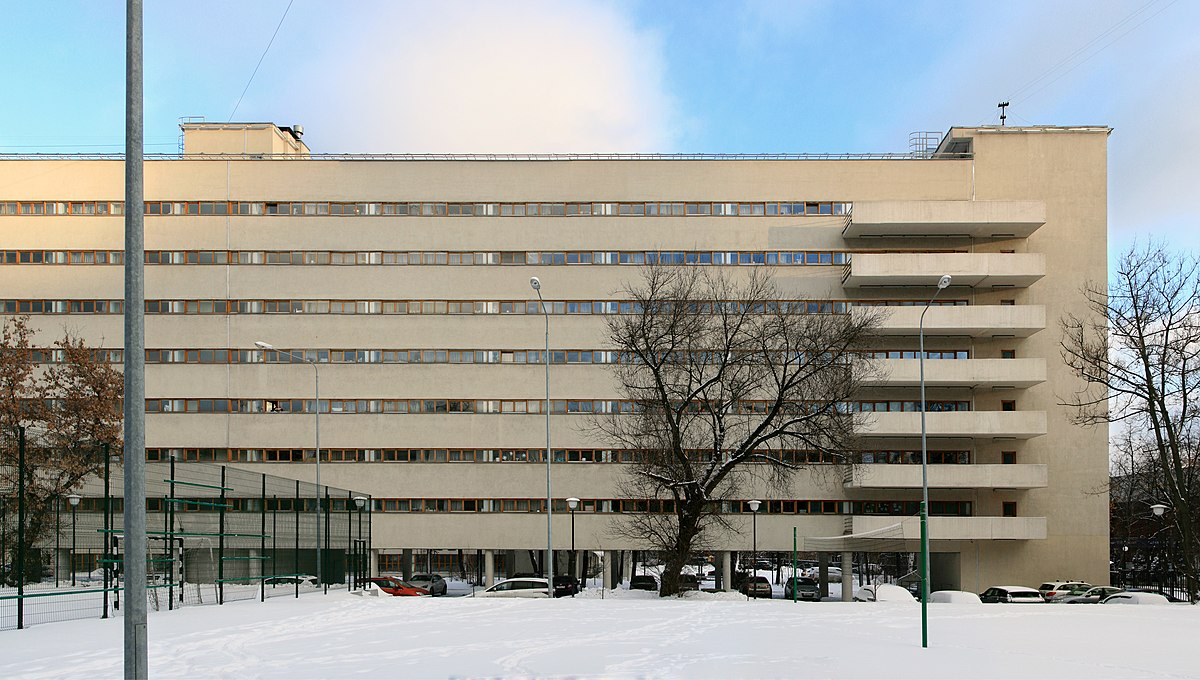
\includegraphics[width=0.9\textwidth]{images/Moscow_Ordzhonikidze8_Y18.jpg}
                    \caption*{Дом-коммуна на ул. Орджоникидзе}
                \end{figure}
            }
        \end{column}
    \end{columns}
\end{frame}
